\documentclass[DM,lsstdraft,toc]{lsstdoc}

% lsstdoc documentation: https://lsst-texmf.lsst.io/lsstdoc.html

% Package imports go here.

\input{aglossary.tex}
\makeglossaries

% Local commands go here.

% To add a short-form title:
% \title[Short title]{Title}
\title{LSST Software Release Management}

% Optional subtitle
% \setDocSubtitle{A subtitle}

\author{%
Leanne P. Guy, Gabriele Comoretto
}

\setDocRef{LDM-672}

\date{\today}

% Optional: name of the document's curator
\setDocCurator{Leanne Guy}

\setDocAbstract{%

This document describes the processes that \gls{LSST} Data Management will adopt for managing
DM Software Products release in order to meet the current and future needs of the \gls{LSST} science program.
These processes will facilitate contrinutions from the science community and ensure proper \gls{LSST} \gls{DM} operations.
}

% Change history defined here.
% Order: oldest first.
% Fields: VERSION, DATE, DESCRIPTION, OWNER NAME.
% See LPM-51 for version number policy.`
\setDocChangeRecord{%
  \addtohist{}{2019-04-22}{Definitions and Requirements}{G. Comoretto}
  \addtohist{}{2018-12-03}{First draft}{Leanne P. Guy, G. Comoretto}
}

\begin{document}

% Create the title page.
% Table of contents is added automatically with the "toc" class option.
\maketitle

% ADD CONTENT HERE ... a file per section can be good for editing
\section{Introduction} \label{sec:intro}

This document prests the release manafgement approach for \gls{LSST} \gls{DM} software products.

First of all, in section \ref{sec:reqs}, the release requirements for the varius  stakeholders are identified.
The release requirements are then consolideated in section \ref{sec:reqdef}.
These requirements are not formal project requirements, as given for example in the \gls{DMS} requirements specification \citeds{LSE-61}, but are nevertheless important to ensure the project's goals.

Based on the consolidated reqirements, a set of policies are derived in section \ref{sec:policy} and guidelines on their applicability is provided in section \ref{sec:noncompliance}.

Finally section \ref{sec:process} goves a high level overview of the release process.


\subsection{Releases Status}\label{sec:sci}

Currently, only the \gls{Science Pipelines} product is released. 
Builds and releases are made on the following time-based cadence:

\begin{itemize}
\item Nightly builds
\item Weekly builds
\item Official releases every 6 months
\end{itemize}

The time needed to consolidate an official release from a weekly build is considerable.
Usually 2 or 3 weeks are sufficient but in some cases it may take more than a month. 
Consequently, by the time a release becomes available to the users, it is already old.
For this reason, users generally prefer to work with weekly builds that are sufficiently stable and include all new functionalities completed in the last week.

The \gls{Science Pipelines} release checklist is documented in \citeds{SQR-016}.
The technical note \citeds{DMTN-106} generalize the process and summarize the technical problems that need to be solve in order that this procedur can be applied to other software products.


\subsection{Policy Applicability} \label{sec:applicability}

This policy shall be applicable to all \gls{DM} software products.

The \gls{DM} software products are defined in the LDM-294. 
The approved product tree is available online at\url{https://ldm-294.lsst.io/ProductTreeLand.pdf}

The policy may also be applicable to other software products development by other \gls{LSST} subsystems.

In case 


\subsection{Definitions} \label{sec:defs}

The relevant definition to be considered when working on release policy and process are given in \citeds{DMTN-106}, section 2.


\newpage
\section{Stakeholders Requirements} \label{sec:reqs}

This section address the questions:

\textbf{Why are DM software releases needed? Who is requesting them ?}

The classic answer to the second questions is that  stakeholders request releases for various reasons.

The following subsections summarize the release requirements on \gls{DM} software products from the different stakeholders' points of view.

It is important to identify these requirements and the corresponding policies during the construction phase, in order to have them consolidated when operations start.

In operations, some of the \gls{LSST} subsystems may no longer exist, for example, \gls{DM} will not exist per se but \gls{DM} software products will still exist under another managerial structure.
The requirements and policies defined here will still be applicable since many of the stakeholders will still expect software releases to be managed following the process consolidated during construction.


\subsection{Release Requirements for the \gls{LSST} Project} \label{sec:lsstreqs}

The main reason for DM to do software releases is to fulfill the project outcome: provide the Data Products.

In order to do that, software releases shall:

\begin{itemize}
\item be available on a time base cadence (every 6 months) during the construction phase,
\item be available when required by a project milestone, in order to be used for the proper validation (commissioning) and operations activities,
\item implement the  functionality needed for the milestone or phase of the project,
\item include third-party software from the Science Community when this is beneficial to the project outcome,
\item carry an appropriate source code license to permit contributions from the Science Community.
\end{itemize}


\subsection{Release Requirements for the \gls{LSST} Science Community} \label{sec:comreqs}

In preparation for working with the \gls{LSST} data products and software during operations, several \gls{LSST} science collaborations have begun using the \gls{DM} software to run data challenges using precursor data or simulations, and to do performance studies. These activities effectively increase the number of beta-testers of \gls{DM} software products, providing valuable feedback to \gls{DM} on the state of the system.

In order to work effectively with the \gls{DM} software while it is still under development, the science community require:
\begin{itemize}
\item timely access new functionality
\item stable public APIs and schemas in order to build software for User-Generated analyses,
\item patches and bug fixes back-ported to the current stable version of the software,
\item include software provided by external contributors in a software release or distribution (due to the collaborative nature of the project).
\end{itemize}


\subsection{Release Requirements for Data Processing in Operations} \label{sec:procreqs}

The \gls{LDF} will be responsible for generating the necessary data products during commissioning and operations.
The \gls{LDF} requires officially released software to be used in production for the various operational activities.
Software releases will be run in production at National \gls{Center} for Supercomputing Applications (\gls{NCSA}), CC-IN2P3 and in Chile, and possibly at independent Data Access Centers (iDACs).

Release frequencies will depend on the processing type:
\begin{itemize}
\item Prompt Processing requires releases to be available very quick, that could happen on a daily bases, especially in the early days (official releases)
 or a  patch release  for a specific problem may be required during the night (this would require sign off from the \gls{AD} for Science \gls{Operations}).
\item \gls{DRP} processing  must be stable for long periods, currently processing is foreseen to take 9 months.  Before such a long processing run the release must be very well tested and any updates extremely well controlled.
\item Image acquisition and header service, which form part of the image acquisition on the mountain will also need strict change control. Releases for this could be on monthly or even lounge timescales - however if there is a problem a patch will be needed immediately.
\end{itemize}

Patch releases need to be provided with a frequency that depends on the type of processing
and on the urgency of the problems to be fixed.


\subsection{Release Requirements for \gls{LSST} Subsystems in \gls{Operations}.} \label{sec:otherreqs}

Other \gls{LSST} subsystem may be consumers of \gls{DM} software products, for example the Telescope \& Site subsystem software makes use of the \gls{DM} software products.
In order for \gls{DM} to be able to respond correctly to the needs of other \gls{LSST} subsystems, it is important to first identify which \gls{DM} software products are used, and how they are used.


\subsection{Release Requirements for Infrastructural Software} \label{sec:infreqs}

A significant subset of \gls{DM} software products are used to provide services to \gls{LSST} science users and staff but are not directly used to generate \gls{LSST} science data products. An example of this is the software that implements the \gls{LSST} \gls{Science Platform} (\gls{LSP}).

Releases of this type of software are typically on their own cadence and need to be adequately tested before deployment to ensure a stable infrastructure.
The releases may be tied to processing milestones if the services or features thereof are required for the processing (e.g. functionality of the workflow service may be required for \gls{Data Release} processing and features in the \gls{LSP} may be needed for \gls{QA} of data products).

Patch releases may need to be provided depending on the urgency and severity of the problems to be fixed.


\subsection{Release Requirements for non-Operational Project Activities} \label{sec:nonopsreqs}

This includes activities done in preparation for operations, such as commissioning,
large scale integration/validation test campaigns, etc. These activities should use use,  as much as possible,  officially released software.

In some cases however, it is necessary to use non-released software, such as release candidates or stable builds.
In all cases, the software used must be clearly identified (Github revision at least), and the distribution/deployment strictly controlled.


\newpage
\section{Requirements Consolidation} \label{sec:reqdef}

The main purpose of this section is to identify all possible release requirements.
In the first subsection a few general requirements are given.
The second subsection summarizes the requirements given by the stakeholders.

A summary overview of the requirements per stakeholder is given at the end of the section.


\subsection{General Requirements} \label{sec:genreq}

The following general requirements are needed in order to properly implement the release process.


\subsubsection{Software Products Identification Requirement} \label{sec:swid}

All \gls{SW} products shall be clearly and unequivocally identifiable in the source repository (GitHub) and documented.

\citeds{DMTN-106} subsection 2.2 (see \ref{sec:defs}) provides a software product definition that can be used as a starting point to identify the DM software products.
The DM product tree provided together with \citeds{LDM-294}, is available at the following link \url{https://ldm-294.lsst.io/ProductTreeLand.pdf}.

This requirement needs to be fulfilled in order to ensure the applicability of the release policy and process.
If the software products are not properly identified, it will not be possible to do releases.


\subsubsection{Software Release Documentation Requirement} \label{sec:reqdoc}

All software releases shall be properly documented with a software release note.


\subsubsection{Software Release Test Requirement} \label{sec:test}

A software release should be fully tested before making it available for use.
The test should be documented in a test report.


\subsection{Stakeholders Requirements} \label{sec:stakeholdersreqs}

The following list of requirements is derived from the above section \ref{sec:reqs}.


\subsubsection{Releases Schedule Requirement} \label{sec:milestone}

Releases on a software product shall be scheduled in advance.

Two types of release schedule can be identified:

\begin{itemize}
\item Functional Based Release Schedule: a release shall provide a requested functionality.
\item Time-Based Release Schedule: a release shall be provided on a specific date or cadence.
\end{itemize}

In both cases, releases can be tight to project milestones.
Additional releases can be requested to the DM-CCB using the RFC mechanism.


\subsubsection{Patch Release Requirement} \label{sec:backport}

It shall be possible to backport a fix on a stable release and provide a patch release including only the backported fix.


\subsubsection{Third-Party Software Inclusion Requirement} \label{sec:thirdsw}

It shall be possible to include in a software product release or distribution release, a software package provided by a third-party contributor.


\subsubsection{Stable public APIs and Schemas Requirement} \label{sec:stable}

Public APIs and schemas shall be stable and follow a well-defined deprecation mechanism in order to give time to the stakeholder to adapt to the new API.


\subsubsection{License Requirement} \label{sec:license}

DM software shall be released with an appropriate license, that permits to use and redistribution of software provided by external collaborators.


\subsection{Requirements Summary Overview} \label{sec:overview}

The following table gives an overview of the release requirements applicable for each stakeholder.

\setlength\LTleft{-0.4in}
\setlength\LTright{-0.5in}
\begin{longtable}{p{2.4cm}p{1.2cm}p{1.4cm}p{1.4cm}p{1.3cm}p{1.3cm}p{1.3cm}p{1.7cm}p{1.3cm}p{1.3cm}}\hline
&
\textbf{SW Ident.}&\textbf{Release Doc.}&\textbf{Release Test}&\textbf{Funct. Based}&\textbf{Time Based}&\textbf{Patch}&\textbf{3rd Party SW}&\textbf{Stable API} &\textbf{License}\\ \hline
\textbf{LSST Project} \ref{sec:lsstreqs}&
YES                     & YES                         & YES                         &  YES                         &  YES                      & YES             & YES                          &  YES.                   & YES   \\ \hline
\textbf{Science Community} \ref{sec:comreqs}&
YES                     & YES                         &                                 &                                   &  YES                     & YES.            & YES                          &  YES.                   & YES   \\ \hline
\textbf{DM Operations} \ref{sec:procreqs}&
YES                     & YES                         & YES                         & YES                           &                              & YES             & YES                          &  YES(?)                &            \\ \hline
\textbf{Other Operations} \ref{sec:otherreqs}&
YES                     & YES                         & YES                         & YES                           &                              & YES             &                                  &  YES(?)                &            \\ \hline
\textbf{Infrastructure} \ref{sec:infreqs}&
YES                     & YES                         & YES                         &                                   &  YES                     & YES             &                                  &  YES                    &            \\ \hline
\textbf{Non Operations} \ref{sec:nonopsreqs}&
YES                     & YES(?)                     & YES(?)                    & YES                           &  YES                     & YES             & YES                          &  YES                    &            \\ \hline
\hline
\end{longtable}
\setlength\LTleft{0in}
\setlength\LTright{0in}




\newpage
\section{Process} \label{sec:process}


The high-level Release Management plan for \gls{DM} is documented in \citeds{LDM-294}, section 3.6. 
In order to avoid duplications, this process should be maintained only in one document.


\subsection{Release Process Definition}

The release process will be as follows:

\begin{itemize}
\item Major and minor releases will be planned and approved by the DM-CCB.
\begin{itemize}
  \item  DM-CCB will provide  a release plan identifying  milestones requiring software releases.
  \item The DM-CCB will monitor and approve or reject the content of each release. DM-CCB will ensure that  all RFCs that impact  release content are properly escalated.
\end{itemize}
\item Any extra releases, major, minor or patch, has to be requested by the release end users to the DM-CCB via \gls{RFC}. The \gls{RFC} shall contain:
\begin{itemize}
  \item the reason for an extra release
  \item the list of features or fixes which are requested to be implemented in the release
  \item the date the release is requested to be available and specify the urgency.
\end{itemize}
\item The DM-CCB will assess the release request involving the relevant T/CAMs and technical contributor affected.
Urgent release request will be approved in 24 hours, non urgent release requests will be approved in one week's time.
\item The release request may be approved or rejected.
\item In case of approval, the following information will be added in a comment to the RFC:
\begin{itemize}
  \item version identification of the release
  \item date the release will be available (an estimation, that may change)
  \item confirm content of the release
\end{itemize}
\item the DM-CCB will monitor the progress of the release's activity and communicate changes in the release date
\end{itemize}


The DM-CCB meets every week.

Technical aspects and roles (who does what) are addressed int following documents:

\begin{itemize}
\item {\bf regular development}: in the \href{https://developer.lsst.io/}{developer guide}
\item {\bf fix porting}: in the \href{https://developer.lsst.io/}{developer guide}
\item {\bf release note documentation}: in the \href{https://developer.lsst.io/}{developer guide} or a different document
\item {\bf release engineering}: in the DMTN-106 (still draft). \href{https://sqr-016.lsst.io/}{SQR-016} is used for the science pipelines release.
\end{itemize}


\subsection{Urgent Releases}

In the case a very urgent release is required, that can't wait a formal approval of the DM-CCB (24 hours),
a quick decision can be taken by the \gls{DMPM} and a requested fix can be implemented and released immediately, if feasible.

However, an \gls{RFC} has to be filed a posteriori, and the DM-CCB is required to assess it.



\appendix

%definitions. This could be moved in the main part pf the document
\section{Definitions} \label{sec:defs}

The following definitions have to be taken in account when defining or working with the release process.


\subsection{Environment} \label{sec:envdef}

An environment is a set of libraries, executables and configurations, that are predefined for a specific context or function.

An environment is usually needed in the following contexts:

\begin{itemize}
\item software development: the environment includes all libraries and tools required to build and debug a software product
\item software test and verification: the environment includes, on top of build and debug tools, additional tools to permit/facilitate the testing and validation activities.
\item operations: the environment shall include only tools required for the execution of the operational products. It shall not contain any build or debug tool. It shall be optimized for the operational activities. \footnote{In case a problem is found in operation the first thing to do is to replicate it in a different environment, where also debug and further analysis is possible.}
\end{itemize}

These are the most common uses of an environment. Additional scenarios can be identified depending on the needs.

In some cases, for simplicity, the same environment is used in development, tests and operations, but this does not justify the inclusion of the environment definition in the Software Product itself.


\subsection{Software Product} \label{sec:swdef}

A Software Product is a component of the subsystem (DM) product tree.

The following activities are done on a SW Product:
\begin{itemize}
\item development activities
\item test activities, usually unit tests and system test
\item release activities
\item packaging activities
\item operational activities, in stand alone mode, in an operational pipeline or as part of a service. Some SW Products are libraries, therefore are not operationally, but used as dependencies by other Software Products.
\end{itemize}

A Software Product shall correspond to a single repository. 
In other  words, there shall be a correspondence \textit{1:1} between Software Products and git packages.
All the Software Product's dependences are different Software Products and therefore released separately.

This is not the case of DM, where a Software Product is comprised of multiple git packages.
The compromised solution in this case is to have a GitHub \textit{metapackage} that identifies the Software Product.
All git packages composing the Software Product are dependencies in a GitHub \textit{metapackage} and released at the same time.
In this case, a git package shall be related only to one Software Product, and it is not by himself a Software Product.
In other words, there is a correspondence \textit{1:many} between Software Product and Git packages. 
There shall never be a \textit{many:many} correspondence.

The following elements should not be part of a Software Product:

\begin{itemize}
\item build tools, otherwise we will have build tools deployed in operations.
\item environment definition, since the environment depends on the final instantiation of the Software Product that are not visible in the development phase.
\end{itemize}

These elements shall follow a parallel development / release process.

Test data should also not be included in a Software Product. However including small datasets for enabling the unit tests is not a bad practice.

The content of this subsection is a \textit{prerequisite} for any release procedure to be applied.


\subsection{Software Release} \label{sec:defrelease}

A software release is a consciously identified tag of a Software Product repository documented with a software release note.
The identifier is usually of the form \texttt{M.n.p}.

The tag in the Github repository and the software release note shall be sufficient to identify the release, and therefore for a developer
to resolve the dependencies, build the binaries and execute the software.

The software release is a monolithic snapshot of the Software Product to be used as is, or in its corresponding binary package(s), by the downstream processes or users.
In theory, it should be possible to identify the release with a checksum calculated automatically on the delivered package.
That checksum can be used to identify the release installed in an environment, or included in a distribution.


\subsection{Third Party Packages}

Third party packages are those packages that are not developed in DM, and follow their own documentation and release process.


\subsection{Binary Packages} \label{sec:swbpkg}

A binary package is a package containing executable for the corresponding release.
It is created by building the SW provided in the release tag.
Binary packages can be created to support multiple platforms (such as Linux, OSX, windows) if required.

In some cases, these packages do not contain compiled binaries, but executable scripts or just text files.

Binaries should be generated only once, and made available for their use by dependent software or for deployment.


\subsection{Distribution} \label{sec:distribution}

A distribution is a collection of well identified binary packages to be deployed together.

A distribution can be used for different purposes:

\begin{itemize}
\item to make available software releases for operations or commissioning
\item to test (integration, validation, operation rehearsals) software releases
\item to provide software releases to external collaborators. In this case source code can be distributed instead of binaries.
\end{itemize}

Distributions may also include non binary packages, build tools, test data or source code, as needed.

Depending on the purpose, the packages included in a distribution may not correspond to a specific software release. 
For example for test purposes, a release candidate can be used instead or, during commissioning, 
it may be necessary to deploy on the fly a package including changes just made in the repository
and identified only by the corresponding revision.



\newpage
\section{DM Software Product Tree}\label{sec:swptree}

Follows the \gls{DM} software product tree, listing all operational \gls{DM} software products.

Full product tree is available in \citeds{LDM-294}.

At May 2019, this list is still a proposal and none of the software products included here are correctly defined.



\begin{figure}
\begin{center}
 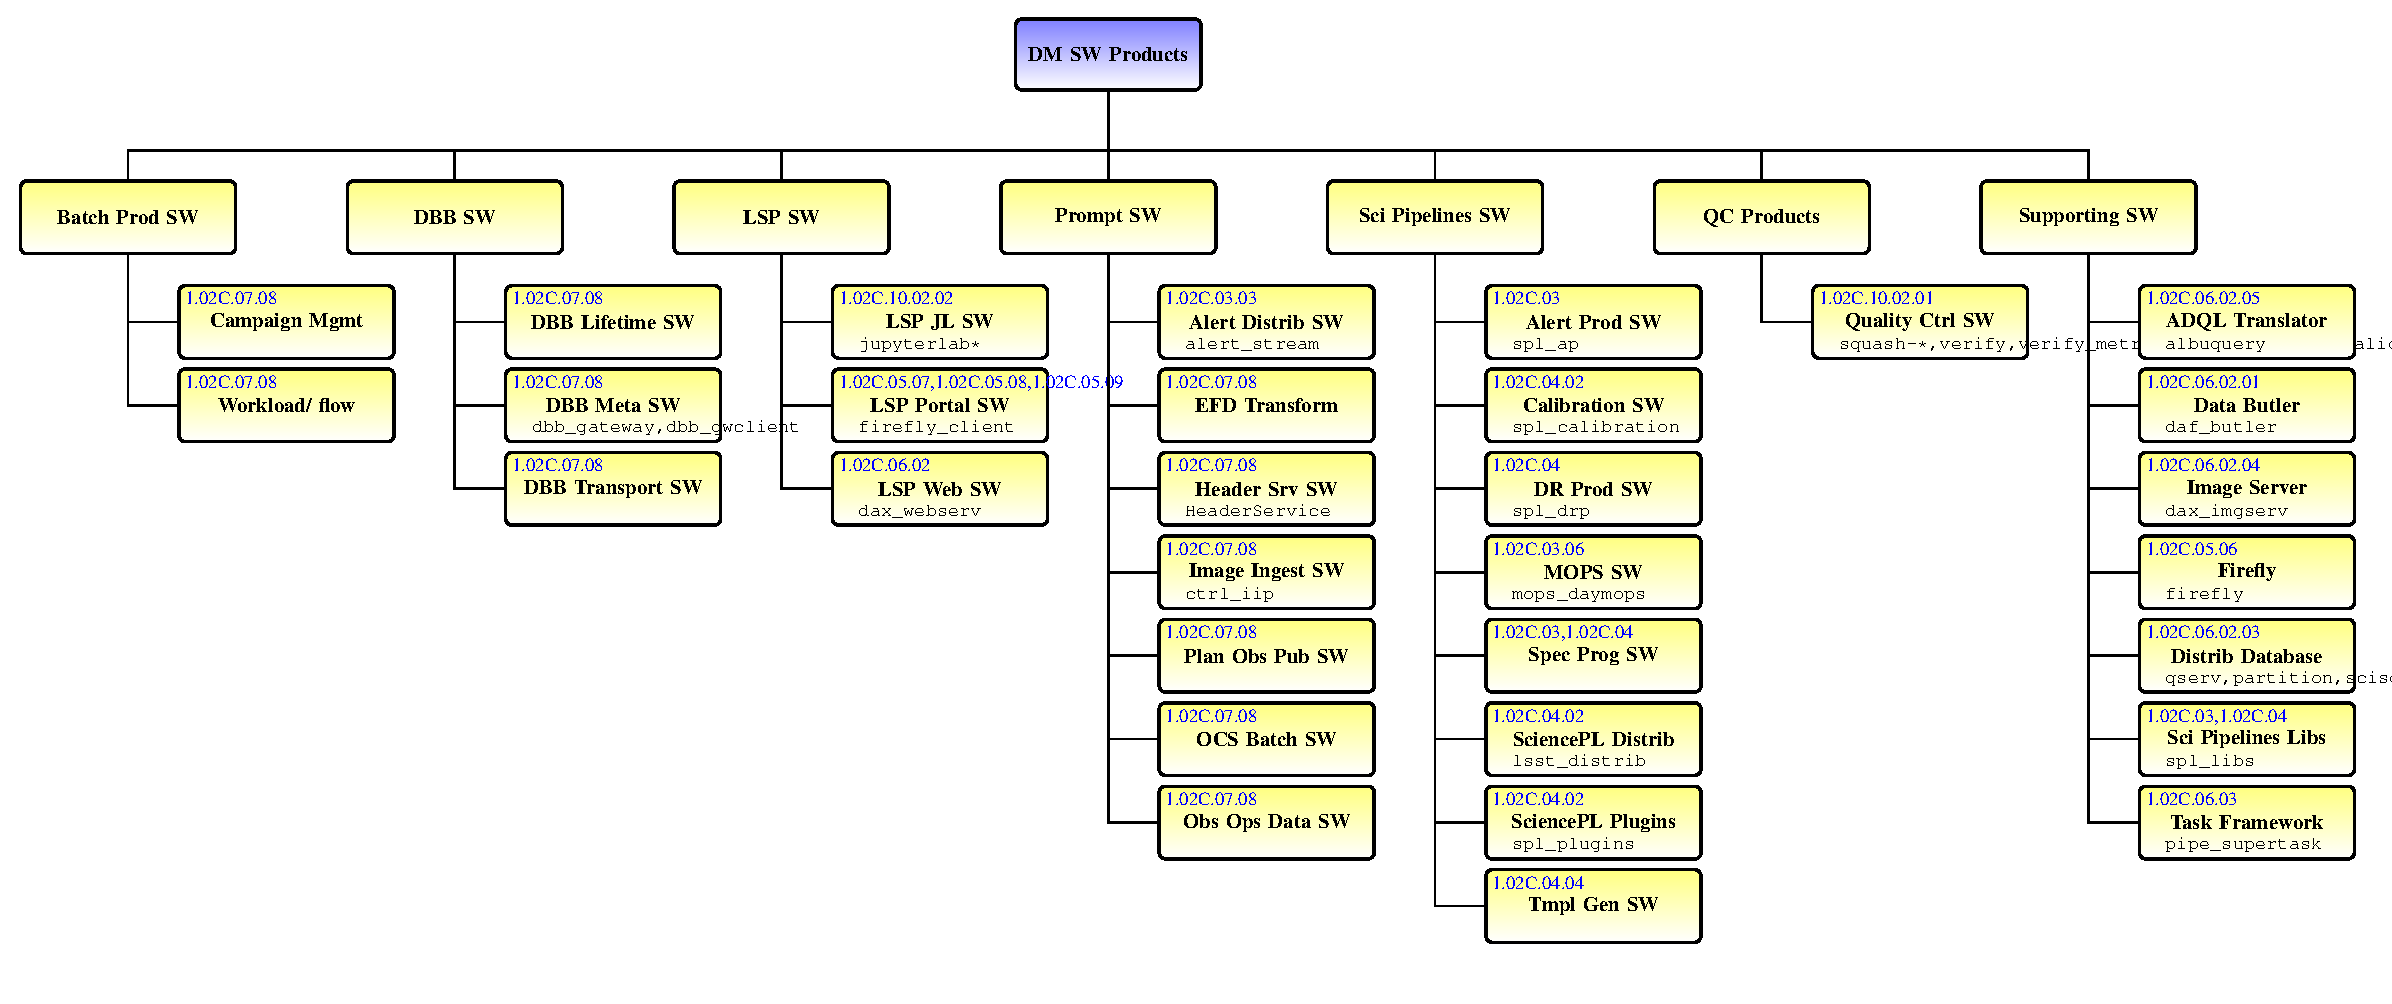
\includegraphics[width=1.1\textwidth]{ProductTreeLand}

 \caption{The \gls{DM} Software product tree.}
 \label{fig:doctree}

\end{center}
\end{figure}

The \textit{Science Pipelines Distribution} is included in the list since it is the only DM product that is currently released.
However this is not really a Software Product but a distribution.
It includes all Science Pipelines Software Products, test data, development and build tools, and everything that is required by the Science Collaborators to contribute to the project.

% Include all the relevant bib files.
% https://lsst-texmf.lsst.io/lsstdoc.html#bibliographies
\section{References} \label{sec:bib}
\bibliography{lsst,lsst-dm,refs_ads,refs,books}

%Make sure lsst-texmf/bin/generateAcronyms.py is in your path
\printglossaries

\end{document}
